\chapter{Architektura rozwiązania}

Niniejszy rozdział przedstawia architekturę rozwiązania, obejmującą zarówno założenia projektowe, jak i koncepcję opracowywanego systemu. Założenia projektowe określają podstawowe wymagania oraz wytyczne, stanowiąc punkt wyjścia dla opracowywanego rozwiązania. Natomiast koncepcja rozwiązania, uwzględniająca zasadnicze założenia, strukturę i logikę działania, stanowi podstawę implementacji rozwiązania.

\section{Założenia projektowe}
Założenia projektowe definiują podstawowe wytyczne dotyczące funkcjonalności i wymagań technicznych tworzonego rozwiązania. Obejmują one m.in. systematyzację danych, wykorzystanie platformy Microsoft 365 oraz optymalizację procesów decyzyjnych.




\subsection{Systematyzacja danych}
Jedną z zasadniczych funkcji omawianej aplikacji jest systematyzacja danych. Arkusze kalkulacyjne przesyłane przez oddział w Wolfsburgu nie posiadają ustandaryzowanej struktury, co negatywnie wpływa na ich czytelność oraz czas potrzebny na analizę.

\noindent Tabela \ref{HeaderComparison} przedstawia różnice w nazwach kolumn na przestrzeni trzech lat.

\renewcommand{\arraystretch}{1.3} % Zwiększenie wysokości komórek
\begin{table}[H] % [t] - tabela bliżej górnej krawędzi strony
   \centering
   \caption{Zestawienie nagłówków kolumn w latach 2022-2024}
   \label{HeaderComparison}
   \makebox[0.925\textwidth][c]{%
      \begin{tabular}{|c|W|W|W|}
         \hline
          & \textbf{2022}            & \textbf{2023}            & \textbf{2024}            \\ \hline
         \multirow{12}{*}{\rotatebox{90}{\parbox{3cm}{\centering \textbf{Nazwy kolumn na   \\przestrzeni lat}}}}
          & Service group            & Service group            & Service group            \\ \cline{2-4}
          & Service main group       & Service main group       & Service main group       \\ \cline{2-4}
          & Service sub group        & Service sub group        & Service sub group        \\ \cline{2-4}
          & Business Service         & Business Service         & Business Service         \\ \cline{2-4}
          & ID                       & ID                       & ID                       \\ \cline{2-4}
          & Business Service Manager & Business Service Manager & Business Service Manager \\ \cline{2-4}
          & Unit of Measurement      & Unit of Measurement      & Resource Unit            \\ \cline{2-4}
          &                          & Settlementtype           & Settlementtype           \\ \cline{2-4}
          & PL70 2022 PLAN EUR w KVA & PL71 2023 PLAN EUR w KVA & PL72 2024 PLAN EUR w KVA \\ \cline{2-4}
          & QTY                      & QTY                      & QTY                      \\ \cline{2-4}
          & PL71 2023 PLAN EUR w KVA & PL72 2024 PLAN EUR w KVA & PL73 2025 PLAN EUR w KVA \\ \cline{2-4}
          & QTY                      & QTY                      & QTY                      \\ \hline
      \end{tabular}
   }
\end{table}

Brak jednolitego formatu danych uniemożliwia również stworzenie spójnej bazy, co ogranicza możliwość ich wykorzystania w systemach automatyzacji procesów biznesowych. Dzięki wdrożeniu omawianego rozwiązania możliwe jest ujednolicenie danych, co pozwala na efektywne nimi zarządzanie i automatyczne przetwarzanie.
\subsection{Archiwizacja danych}
Utworzenie bazy danych gromadzącej informacje o wcześniejszych działaniach realizowanych w ramach projektowanego systemu stanowi istotny element zapewniający ciągłość procesów decyzyjnych. Dzięki systematycznej archiwizacji nowi użytkownicy mogą szybko zapoznać się z przebiegiem procedur i lepiej zrozumieć kontekst dotychczas podejmowanych decyzji. Dostęp do zasobów historycznych nie tylko skraca czas potrzebny na pełne wdrożenie w funkcjonowanie systemu, lecz także usprawnia przetwarzanie danych bieżących.
\subsection{Interfejs przyjazny dla użytkownika}
\begin{comment}Dedykowane narzędzie z prostym i intuicyjnym interfejsem znacząco ułatwia nawigację po bazie danych, eliminując problemy związane z tradycyjnymi rozwiązaniami, takimi jak arkusze kalkulacyjne. \end{comment}

Dzięki dedykowanemu narzędziu z prostym i intuicyjnym interfejsem, nawigacja po bazie danych jest znacznie prostsza, a problemy związane z używaniem arkuszy kalkulacyjnych zostają wyeliminowane. Przyjazny dla użytkownika interfejs oznacza:
\begin{itemize}
    \item \textbf{Prostotę:} nieskomplikowany układ umożliwia szybkie odnalezienie potrzebnych informacji
    \item \textbf{Przejrzystość:} dane są zaprezentowane w sposób czytelny, z jasno określonymi polami i etykietami
    \item \textbf{Przydatne funkcje:} filtrowanie i wyszukiwanie danych wspierają efektywność pracy
\end{itemize}
Klarowny układ i czytelność interfejsu pozwalają użytkownikowi skupić się na konkretnej usłudze, co minimalizuje ryzyko pomyłek, takich jak błędne interpretowanie danych lub wybór niewłaściwego wiersza.

Takie podejście nie tylko zwiększa efektywność pracy, ale również poprawia komfort użytkowników, dzięki czemu procesy związane z analizą i zarządzaniem danymi stają się bardziej zrozumiałe i mniej podatne na błędy.
\subsection{Użycie pakietu Microsoft 365}
\begin{comment}


Wykorzystanie platformy Power\footnote{Platforma Power (\english{Power Platform}) -- Składowa pakietu Microsoft 365. Zawiera ona takie programy jak Power Apps, Power Automate czy Power BI.} w połączeniu z Sharepoint, pozwala na utworzenie w pełni funkcjonalnego rozwiązania, zachowując spójność danych dzięki integracji poszczególnych składników pakietu.

Aby korzystanie z aplikacji było możliwe, użytkownicy muszą mieć dostęp do potrzebnych usług oraz licencje. W przypadku omawianego pakietu, każdy z pracowników, ma do niego dostęp. Pozwala to na uniknięcie dodatkowych kosztów.

Niestety użyty pakiet, nie jest dostępny w najbardziej rozbudowanym wariancie. Wprowadza to pewne ograniczenia, ponieważ brakuje w nim oprogramowania do tworzenia i zarządzania rozbudowanymi bazami danych o złożonej strukturze (takie możliwości daje między innymi \emph{Microsoft Azure}).
Sharepoint pozwala jedynie na utworzenie prostej bazy danych opierającej się o wcześniej opisane listy.  Głównym problemem było ograniczenie związane z brakiem możliwości tworzenia relacji między kilkoma listami, co znacząco utrudniało zarządzanie danymi o złożonej strukturze.

\end{comment}

Wykorzystanie platformy Power\footnote{Platforma Power (\english{Power Platform}) -- składowa pakietu Microsoft 365, w skład której wchodzą takie programy, jak Power Apps, Power Automate czy Power BI.} w połączeniu z Sharepoint, pozwala na utworzenie w pełni funkcjonalnego rozwiązania, zachowując spójność danych dzięki integracji poszczególnych składników pakietu.

Aby korzystanie z aplikacji było możliwe, użytkownicy muszą mieć dostęp do potrzebnych usług oraz licencji. W przypadku omawianego pakietu, każdy z pracowników ma do niego dostęp, co pozwala uniknąć dodatkowych kosztów.

Wykorzystany pakiet nie jest dostępny w najbardziej rozbudowanym wariancie, co wprowadza pewne ograniczenia, ponieważ nie zawiera oprogramowania do tworzenia i zarządzania rozbudowanymi bazami danych o złożonej strukturze (takie możliwości daje między innymi \emph{Microsoft Azure}).
Sharepoint pozwala jedynie na utworzenie prostej bazy danych opierającej się o wcześniej opisane listy.


%\customnote{ //To chyba do implementacji // Głównym problemem było ograniczenie związane z brakiem możliwości tworzenia relacji między kilkoma listami, co znacząco utrudniało zarządzanie danymi o złożonej strukturze.}

\subsection{Optymalizacja}
Głównym celem implementowanego rozwiązania jest usprawnienie procesu decyzyjnego poprzez zwiększenie efektywności analizy i przetwarzania danych. Dzięki automatyzacji czas potrzebny na podjęcie decyzji zostaje znacząco skrócony, co przekłada się na większą wydajność całego procesu.

Dzięki wprowadzeniu mechanizmów automatyzacji biurowej możliwe jest zmniejszenie liczby osób zaangażowanych w realizację procesu, co może przyczynić się do ograniczenia kosztów operacyjnych i lepszej organizacji personelu w przedsiębiorstwie.
\section{Koncepcja rozwiązania}
\sectionauthor{R. Wolniak}
W niniejszym podrozdziale przedstawiona została koncepcja rozwiązania problemu automatyzacji procesu decyzyjnego. Na podstawie przeprowadzonej analizy wymagań oraz istniejących ograniczeń, zaproponowano kompleksowe podejście do realizacji systemu.

Całość rozwiązania podzielono na cztery główne etapy:
\begin{itemize}
    \item utworzenie dedykowanej bazy danych,
    \item opracowanie mechanizmu importu danych z arkuszy kalkulacyjnych,
    \item przygotowanie formularzy do obsługi procesu,
    \item automatyzacja generowania raportów.
\end{itemize}

Przyjęte rozwiązanie ma na celu usprawnienie procesu przy zachowaniu jego dotychczasowej logiki biznesowej. Szczegółowy opis realizacji poszczególnych etapów został przedstawiony w kolejnych podrozdziałach.
\subsection{Baza danych}

Do przechowywania danych wykorzystano listy programu SharePoint. Pomimo tego, że nie jest to dedykowane rozwiązanie bazodanowe, wybór ten podyktowany został wymaganiami integracji z istniejącą infrastrukturą.

\subsubsection{Struktura bazy danych}
\label{Subsec: StrukturaBazyDanych}
W wyniku analizy danych historycznych zidentyfikowano elementy kluczowe dla procesu indykacji. Na tej podstawie zaprojektowano strukturę składającą się z trzech powiązanych ze sobą list:

\begin{itemize}
  \item \textbf{Lista usług} -- zawierająca podstawowe, niezmienne informacje o serwisach,
  \item \textbf{Lista kwot} -- przechowująca dane odnośnie cen i liczbie licencji, które zmieniają się raz do roku,
  \item \textbf{Lista indykacji} -- gromadzi informacje w obrębie jednej indykacji.
\end{itemize}
\subsubsection{Atrybuty danych}
Na podstawie analizy wymagań oraz dotychczasowego procesu, zdefiniowano następujący zestaw atrybutów, które powinna zawierać baza danych:

\begin{multicols}{3}
  \begin{itemize}
    \item Service group
    \item Service main group
    \item Service sub group
    \item Business Service
    \item Instruction link
    \item ID
    \item Business Service Manager
    \item Unit Of Measurement
    \item Settlement Type
    \item Current Year Plan EUR
    \item Quantity Current Year
    \item Next Year Plan EUR
    \item Quantity Next Year
    \item Year
    \item MPK
    \item Difference
    \item Indication Number
    \item Comment Intern
    \item Comment Date
    \item Comment Author
    \item Comment PZ to WOB
    \item Comment BSM
    \item Comment K-DES
    \item Decision
    \item Final comment
  \end{itemize}
\end{multicols}
Powyższy zestaw atrybutów został opracowany na podstawie analizy danych historycznych z poprzednich lat (przedstawionych w Tabeli \ref{HeaderComparison}). Wybrane pola reprezentują najczęściej występujące informacje w procesie indykacji, uzupełnione o dodatkowe atrybuty niezbędne do efektywnego funkcjonowania procesu, takie jak pola komentarzy czy decyzji.

\subsubsection{Model powiązań}

\begin{figure}[h]
  \makebox[0.925\textwidth][c]{
    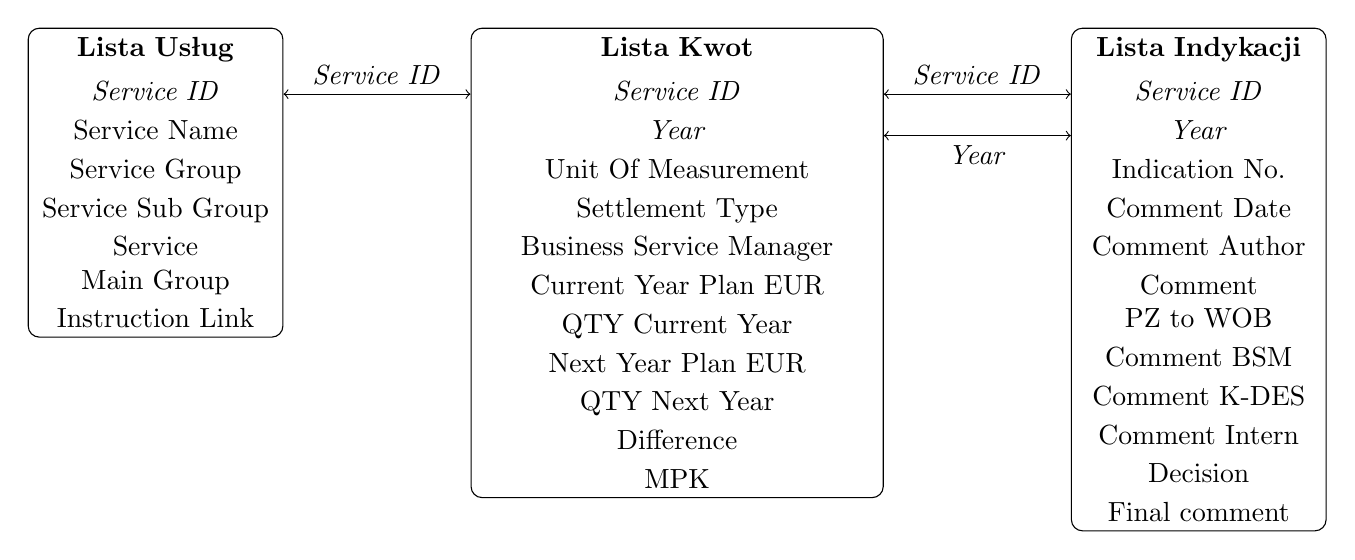
\begin{tikzpicture}

      \tikzstyle{ListBlock} = [
      rectangle,
      rounded corners,
      minimum width=3cm,
      minimum height=1cm,
      text centered,
      draw=black,
      fill=white,
      anchor=north
      ]

      \node (ListaUslug) [ListBlock, text width=3cm] at (0,0) {
        \textbf{Lista Usług}\\[4pt]
        \textit{Service ID}\\[2pt]
        Service Name\\[2pt]
        Service Group\\[2pt]
        Service Sub Group\\[2pt]
        Service Main Group\\[2pt]
        Instruction Link\\[2pt]
      };

      \node (ListaKwot) [ListBlock, text width=5cm]
      at ([xshift=5cm] ListaUslug.north east) {
        \textbf{Lista Kwot}\\[4pt]
        \textit{Service ID}\\[2pt]
        \textit{Year}\\[2pt]
        Unit Of Measurement\\[2pt]
        Settlement Type\\[2pt]
        Business Service Manager\\[2pt]
        Current Year Plan EUR\\[2pt]
        QTY Current Year\\[2pt]
        Next Year Plan EUR\\[2pt]
        QTY Next Year\\[2pt]
        Difference\\[2pt]
        MPK\\[2pt]
      };

      \node (ListaIndykacji) [ListBlock, text width=3cm]
      at ([xshift=4cm] ListaKwot.north east) {
        \textbf{Lista Indykacji}\\[4pt]
        \textit{Service ID}\\[2pt]
        \textit{Year}\\[2pt]
        Indication No.\\[2pt]
        Comment Date\\[2pt]
        Comment Author\\[2pt]
        Comment PZ to WOB\\[2pt]
        Comment BSM\\[2pt]
        Comment K-DES\\[2pt]
        Comment Intern\\[2pt]
        Decision\\[2pt]
        Final comment\\[2pt]
      };

      \draw [<->] ([yshift=-2em-4pt]ListaUslug.north east) -- node[anchor=south]{\textit{Service ID}} ([yshift=-2em-4pt]ListaKwot.north west);
      \draw [<->] ([yshift=-2em-4pt]ListaKwot.north east) -- node[anchor=south]{\textit{Service ID}} ([yshift=-2em-4pt]ListaIndykacji.north west);
      \draw [<->] ([yshift=-3.5em-4pt]ListaKwot.north east) -- node[anchor=north]{\textit{Year}} ([yshift=-3.5em-4pt]ListaIndykacji.north west);

    \end{tikzpicture}}
  \caption{Schemat relacji między listami.}
  \label{SchematList}
\end{figure}

Model danych przedstawiony na Rysunku \ref{SchematList} został zaprojektowany z uwzględnieniem następujących założeń:

\begin{itemize}
  \item \emph{Lista usług} pełni rolę centralnego rejestru serwisów, zawierając ich podstawową charakterystykę,
  \item \emph{Lista kwot} umożliwia śledzenie zmian w wymiarze finansowym na przestrzeni lat,
  \item \emph{Lista indykacji} przechowuje historię procesu decyzyjnego wraz z towarzyszącymi komentarzami i ustaleniami.
\end{itemize}




\subsection{Dodawanie informacji do bazy danych}
Po ustaleniu struktury danych wykorzystywanych przez system, należało określić w jaki sposób informacje z arkuszy kalkulacyjnych będą umieszczane w bazie danych.

Głównym problemem na tym etapie jest brak systematycznej organizacji danych zawartych w arkuszach programu Excel co prowadzi do braku kompatybilności z zaprojektowaną bazą danych. 
Zdecydowano się na utworzenie dedykowanego ekranu w aplikacji, który odpowiada za poprawne przetworzenie danych przy asyście użytkownika w celu uniknięcia błędów.

Pierwszym krokiem jest tymczasowe umieszczenie pliku Excel w folderze znajdujacym się we wspólnej przestrzeni roboczej programu Sharepoint. Dzięki temu, dokument jest dostępny dla innych systemów wykorzystanych do jego przetwarzania. Niestety pomimo możliwości otwarcia pliku przez inne systemy, dane w nim zawarte nie były widoczne. Jak się okazało, większość systemów jest w stanie odczytać informacje pogrupowane w \emph{tabele programu Excel}\footnote{W programie Excel tabelę trzeba osobno zadeklarować np. ręcznie zaznaczając zakres komórek a następnie wybierając opcję \emph{Narzędzia główne}$\to$\emph{Fromatuj jako tabelę}}.

Do rozwiązania tego problemu użyto skryptu pakietu Office, który działa wewnątrz arkusza a co za tym idzie ma bezpośredni dostęp do wszystkich informacji w nim zawartych. Skrypt ten oprócz tworzenia tabeli o dynamicznym rozmiarze, usuwa puste kolumny, które czasem były obecne wśród danych. Utworzony algorytm jest w stanie określić początek tabeli oraz jej wielkość zależną od liczby wierszy oraz kolumn, bez uwzględniania zbędnych informacji.

W celu przystosowania informacji z pliku do bazy danych, zdecydowano się na zastosowanie formularza do walidacji nazw kolumn. Formularz ten pobiera nazwy istniejących kolumn w zapisanym arkuszu i pozwala przypisać do nich nazwy z predefiniowanej listy zawierającej nagłówki znajdujące się w listach Sharepoint. Aktualne nazwy również pobierane są przy pomocy wcześniej opisanego skryptu.

Po usystematyzowaniu struktury użytkownik wybiera rok oraz numer indykacji, której dotyczy wgrywany arkusz. Następnie wszystkie informacje są przekazywane do \emph{flow} programu \emph{Power Automate}, które przypisuje je do odpowiednich listach bazy danych upewniając się, że nie powstają duplikaty.

Zdecydowano, że opisywany ekran będzie posiadał dodatkowy formularz odpowiedzialny za przypisywanie numerów \emph{MPK} dla nowych serwisów. Jest to bardzo ważne ponieważ numer ten okeśla, który obszar zajmuje się rozpatrzeniem usługi. W przypadku usług rozpatrywanych w latach poprzednich numer ten jest przepisywany aby ograniczyć liczbę wypełnianych danych. Oczywiście jest możliwość edycji istniejącego wcześniej numery w razie potrzeby. 
\subsection{Interfejs procesu decyzyjnego}
Interfejs obsługi procesu decyzyjnego został podzielony na dwa współpracujące ze sobą ekrany. Takie rozwiązanie pozwala na zachowanie przejrzystości prezentowanych informacji przy jednoczesnym zapewnieniu dostępu do wszystkich niezbędnych funkcjonalności.

\subsubsection{Ekran nawigacyjny}
Pierwszy ekran pełni rolę panelu nawigacyjnego, prezentującym kluczowe informacje dotyczące usługi:
\begin{itemize}
    \item Service Name -- nazwa serwisu,
    \item Service ID -- unikalny identyfikator usługi,
    \item MPK -- numer określający miejsce powstawania kosztów,
    \item Decision -- aktualny status decyzji.
\end{itemize}
Ponadto użytkownicy będą mieli możliwość filtrowania i wyszukiwania serwisów według następujących kryteriów:
\begin{itemize}
    \item wyszukiwanie serwisów względem ID,
    \item wyszukiwanie serwisów względem nazwy,
    \item filtrowanie według przypisanych numerów MPK,
    \item filtrowanie według statusu decyzji (\emph{Accepted}, \emph{Not Accepted}, \emph{No Status}).
\end{itemize}

\subsubsection{Ekran szczegółowy}
Po wybraniu serwisu z listy, użytkownik zostaje przekierowany do ekranu szczegółowego, który składa się z trzech głównych sekcji:
\begin{itemize}
    \item \textbf{Podgląd danych historycznych} -- prezentuje on zarówno ogólne informacje o serwisie zbierane na przestrzeni lat, jak i szczegóły dotyczące poszczególnych indykacji.
    \item \textbf{Formularz decyzyjny} -- zestaw pól do wprowadzenia informacji o bieżącej indykacji. Składają się na niego:
    \begin{itemize}
        \item rok (wartość domyślna: bieżący),
        \item numer indykacji (wartość domyślna: kolejny wolny numer),
        \item autor (wartość domyślna: zalogowany użytkownik),
        \item komentarze (wewnętrzny, BSM, K-DES),
        \item decyzja (wartość domyślna: poprzednia decyzja).
    \end{itemize}
    
\end{itemize}
\subsection{Generowanie raportu}
Ostatnim etapem cyklu obsługi procesu jest generowanie raportu, następnie przesyłanego do zakładu w Wolfsburgu w celu dalszych konsultacji. Raport jest tworzony na podstawie danych przechowywanych na listach SharePoint, co zapewnia spójność i aktualność informacji.

W dedykowanym oknie aplikacji użytkownik będzie mieć możliwość wyboru odpowiedniego roku oraz etapu (numer indykacji). Na podstawie tych informacji, system przetworzy podane kryteria, aby zgromadzić odpowiednie dane z różnych źródeł.

Kolekcja\footnote{Kolekcja (Power Apps) -- tymczasowy zbiór danych, przechowywanych lokalnie w aplikacji, umożliwiający zarządzanie rekordami podczas jej działania.} danych, utworzona na podstawie wybranych kryteriów, połączy dane z trzech list sharepointowych. Dzięki temu możliwe będzie skonsolidowanie danych w jedną, spójną strukturę, która zawierać będzie wszystkie niezbędne informacje do sporządzenia raportu. Utworzone zostaną mechanizmy wyszukiwania, które umożliwią powiązanie identyfikatorów usług z odpowiadającymi im rekordami, co zapewni integralność zgromadzonych danych.

Dodatkowo, w tym samym oknie aplikacji umożliwiony zostanie użytkownikowi dostęp do podglądu zgromadzonych danych w formie tabeli. Umożliwi to weryfikację poprawności i kompletności informacji przed wygenerowaniem raportu. Po zatwierdzeniu danych, system przekaże zgromadzoną kolekcję do Power Automate, gdzie zostaną one zmodyfikowane, w celu przygotowania raportu w odpowiednim formacie (tj. w formacie arkusza kalkulacyjnego \emph{Excel}) do odesłania.


